\documentclass[12pt]{article}
\usepackage[top=1in,bottom=1in,left=1in,right=1in]{geometry}
\usepackage{alltt}
\usepackage{array}	
\usepackage{graphicx}
\usepackage{tabularx}
\usepackage{verbatim}
\usepackage{setspace}
\usepackage{listings}
\usepackage{amssymb,amsmath, amsthm}
\usepackage{qtree}
\usepackage{hyperref}
\usepackage{oz}
\usepackage[cc]{titlepic}
\usepackage{fancyvrb}
\usepackage{epstopdf}
\usepackage{soul}
\graphicspath{ {./figures/} }

\title{Concordia University\\
Department of Computer Science and Software Engineering\\
\textbf{SOEN 331-S: Formal Methods\\for Software Engineering}\\
\ \\
\textbf{Template for Assignment 4:\\Temporal Logic}}
\author{\textbf{Witnick-Hans Joseph}\\
		\texttt{ID: 29348743}\\
		\textbf{Alexandra Zana}\\
		\texttt{ID: 40131077}\\
		\textbf{Alexandre Eid}\\
		\texttt{ID: 40155833}
\ \\}
\date{\today}

\begin{spacing}{1.5}
\begin{document}
\maketitle

\newpage

\section{Problem 1 (46 pts): Analyzing program behavior}

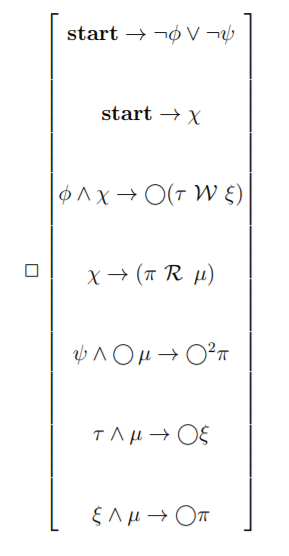
\includegraphics{p1-model.png}

\begin{enumerate}

	\item (36 pts) Visualize all models of behavior.

	\item (10 pts) Specify conditions (models of behavior), if any exist, under which the program\
	can terminate. If none exist, please indicate so.
		
\end{enumerate}

\begin{figure}[ht]
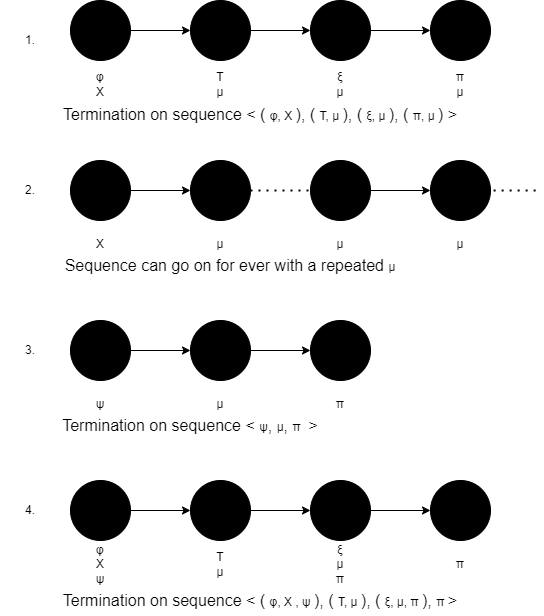
\includegraphics[scale=0.725]{p1.png}
\end{figure}
\newpage

\section{Problem 2 (54 pts) \\Interpreting and visualizing temporal expressionsogram behavior}

Interpret and visualize each of the following temporal expressions:

\end{spacing}

\end{document}